\AtBeginSection[]
{
  \begin{frame}<beamer>
    \frametitle{Examples \thesection}
    \tableofcontents[currentsection]
  \end{frame}
}
\begin{frame}

\frametitle{Need of action}
    \centering
       \begin{tikzpicture} %[spy using overlays]
        \node (pic1) [inner sep=-30pt] {\includegraphics[height=0.588\textheight]{images/SDGs.png}};
% \only<2>{\spy[overlay,width=7cm,height=2cm,magnification=2] on (0,0) in node[] at (2,-3);}
\node [anchor=west, xshift=1.0cm, align=left] at (pic1.south east) {Sustainable \\ Development \\  Goals (SDGs)};

\node (pic2) [inner sep=0pt, anchor=south, yshift=.4cm, xshift=1.5cm, rotate=-20] at (pic1.east) {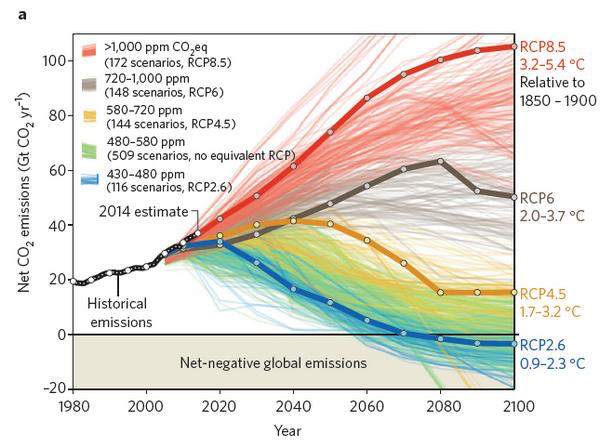
\includegraphics[width=0.3\textwidth]{images/rcps.jpg}}; %
\node [anchor=south, yshift=-.5pt, rotate=-20, align=left] at (pic2.north) {Representative\\ Carbon\\Pathways (RCPs)};

\node (pic3) [inner sep=0pt, anchor=south, xshift=-40pt, rotate=15] at (pic1.north west) {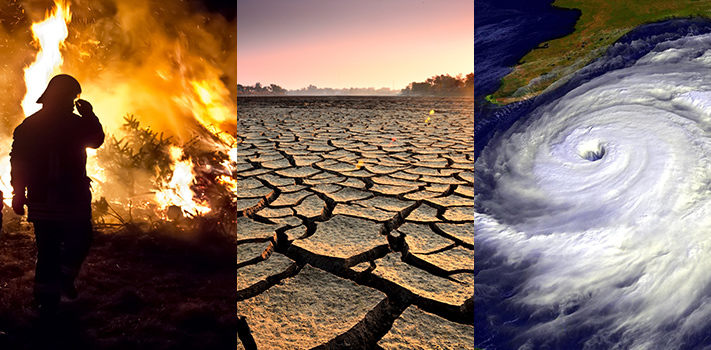
\includegraphics[width=0.5\textwidth]{images/1320_effects-image.jpg}};
\node [anchor=south, rotate=15] at (pic3.north) {\href{https://climate.nasa.gov/effects/}{nasa.gov/effects}};

\node (pic4) [inner sep=0pt, anchor=east, rotate=-5] at (pic1.south west) {\includegraphics[width=0.5\textwidth]{images/Yaounde-flooding.jpg}};
\node [anchor=south, rotate=-5] at (pic4.north) {\href{http://www.cameroonintelligencereport.com/french-cameroun-hundreds-evacuated-as-flooding-hits-yaounde/}{Cameroon Flood at 27.02.2018}};

       \end{tikzpicture}
\end{frame}


\begin{frame}

\frametitle{Growing amount of available data}

\begin{center}
 \includegraphics[width=\textwidth,keepaspectratio=true]{./images/gbif-data-portal-ecpgr-working-group-20170316-5-1024.jpg}
 % gbif-data-portal-ecpgr-working-group-20170316-5-1024.jpg: 0x0 pixel, 300dpi, 0.00x0.00 cm, bb=
\end{center}
\href{https://www.gbif.org/}{Global Biodiversity Facillity}

\end{frame}



\begin{frame}

\frametitle{Predicted EO-data availability for Australia}

\begin{center}
 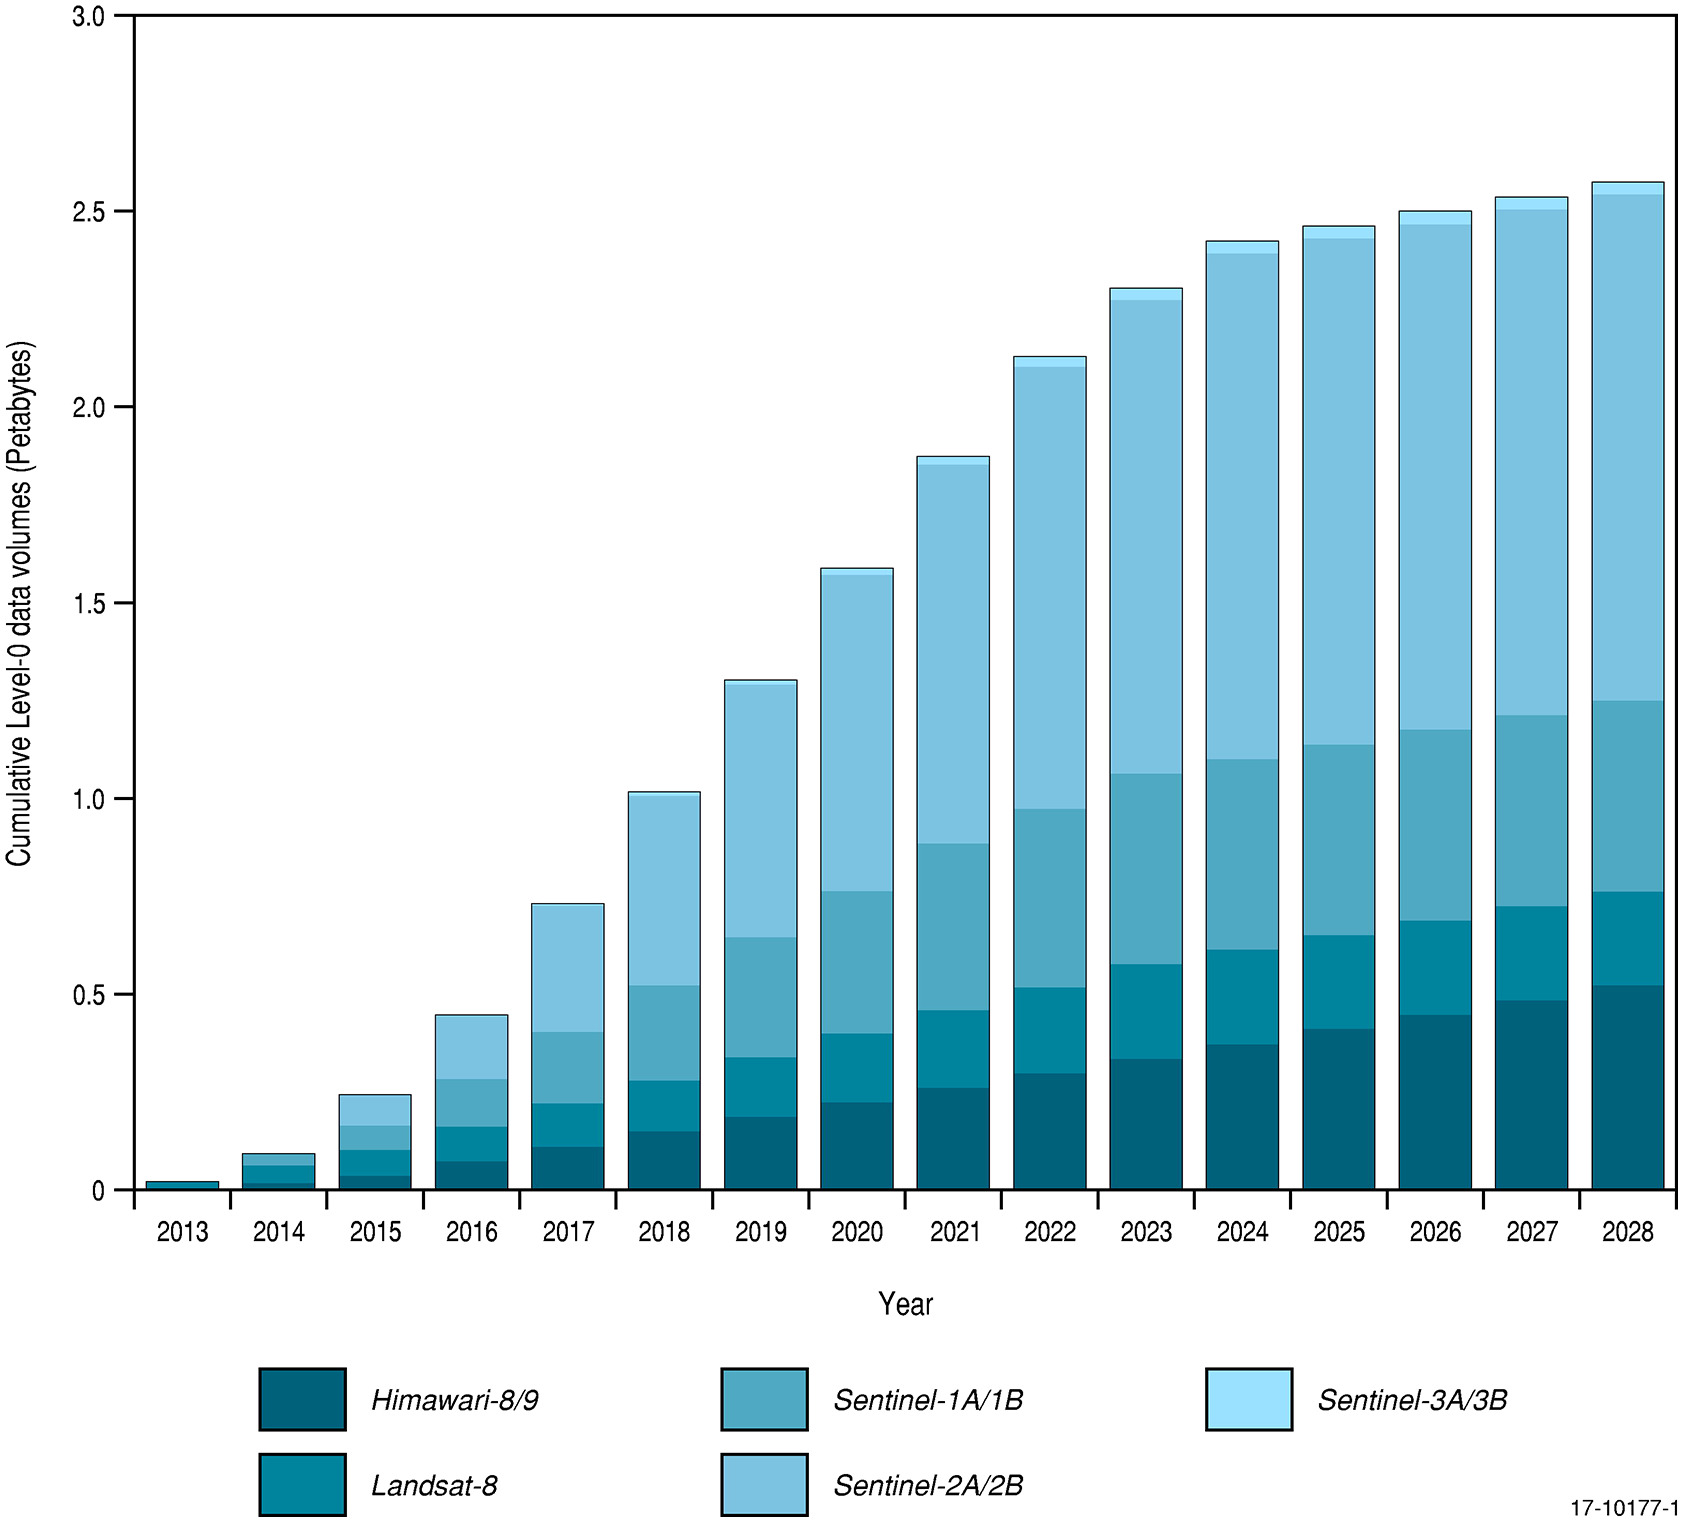
\includegraphics[height=0.8\textheight]{./images/eo-dataamount_australia.jpg}
 % earth-on-aws-nextgeneration-open-data-platforms-24-1024.jpg: 0x0 pixel, 300dpi, 0.00x0.00 cm, bb=
\end{center}

\href{http://nci.org.au/services/virtual-laboratories/australian-geoscience-data-cube/}{Australian Geoscience Data Cube}

\end{frame}

\begin{frame}

\frametitle{Global Climate Model Data Availability}

\begin{columns}[T] % align columns
\begin{column}{.4\textwidth}
	\vspace{1cm}
  \begin{tikzpicture}[scale=0.8]
	\begin{axis}[
	  symbolic x coords={CMIP 1,CMIP 2,CMIP 3,CMIP 4,CMIP 5,CMIP 6},
	  xtick=data,
      ylabel={Peta-Byte},
      ylabel near ticks,
	  ]
 	  \addplot[ybar,fill=blue] coordinates {
	  (CMIP 1,  0.0000001)
 	  (CMIP 2,  0.00005)
 	  (CMIP 3,  0.035)
 	  (CMIP 4,  )
 	  (CMIP 5,  3)
 	  (CMIP 6,  15)
 	  };
	\end{axis}
  \end{tikzpicture}
\end{column}%
\hfill%
\begin{column}{.38\textwidth}
\textbf{CMIP 1:}  ~1 GB\\ % Idealized simulations of present-day climate 
\textbf{CMIP 2:} ~500 GB\\ % Idealized simulations of future climate changes
\textbf{CMIP 3:} ~35 TB\\%  : CMIP3/CMIP2 = 70) More realistic simulations (2004 – present) 
\textbf{CMIP 4:} Not existing\\
\textbf{CMIP 5:} ~3.5 PB (multi-model archive)\\ % ( including replicas, CMIP5/CMIP3 = 100)\\
\textbf{CMIP 6:} currently 10-20 PB as "ESGF" Data (real existing 10time more) \\

************************************\\
IPCC 1 : 1990\\
IPCC 2 : 1995\\
IPCC 3 : 2001\\
IPCC 4 : 2007\\
IPCC 5 : 2014\\
IPCC 6 : --> $\sim$ 2019\\
**************************\\
Global Land Outlook: 2017 \\
(Report UNCCD)
\end{column}%
\end{columns}
% % 
\vspace{0.5cm}
\href{https://cmip.llnl.gov/}{CMIP = Coupled Model Inter-comparison Project}\\
\href{http://www.ipcc.ch/}{IPCC = Intergovernmental Panel of Climate Change}

\end{frame}

\begin{frame}

\frametitle{ Global internet speed (access to information)  }

\begin{center}
 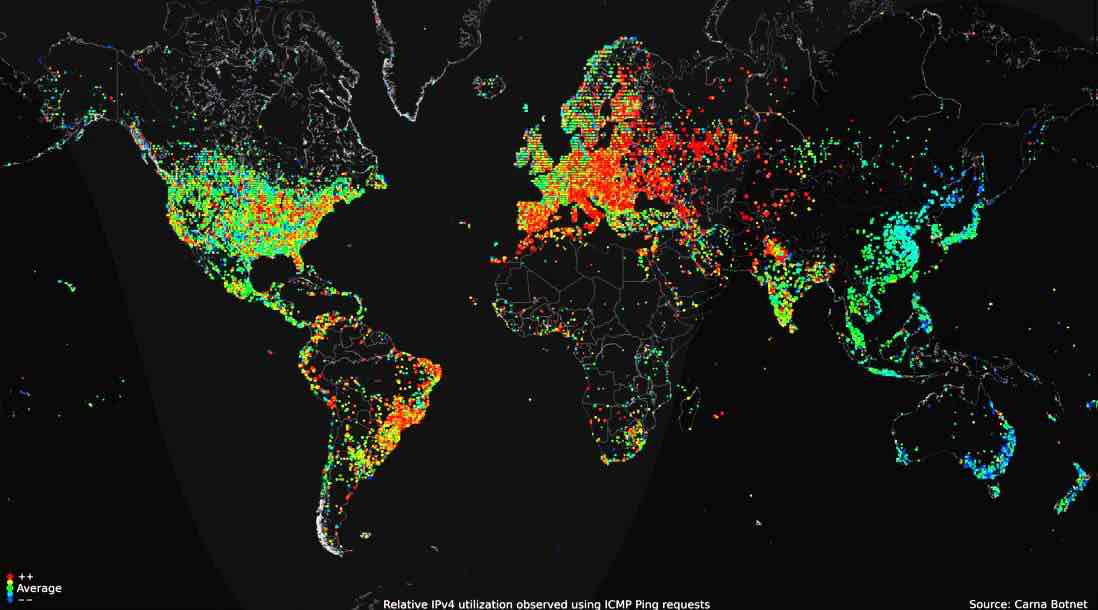
\includegraphics[width=\textwidth,keepaspectratio=true]{./images/internet-users-map-1.jpg}
 % internet-users-map-1.jpg: 0x0 pixel, 300dpi, 0.00x0.00 cm, bb=
\end{center}
\href{https://fossbytes.com/top-10-countries-having-the-fastest-average-internet-speed/}{Global Internet Speed (fossbytes.com)}

\end{frame}

\begin{frame}

\frametitle{The Big Data Problem - Download and Process at home }

\begin{tikzpicture}[
  remember picture,
  overlay,
  expl/.style={draw=orange,fill=orange!30,rounded corners,text width=0.6cm},
  arrow/.style={orange!30,ultra thick,->,>=latex}
]

\node[anchor=south west,inner sep=0]
  (worldmap)
  at (-1,-4.2)
  {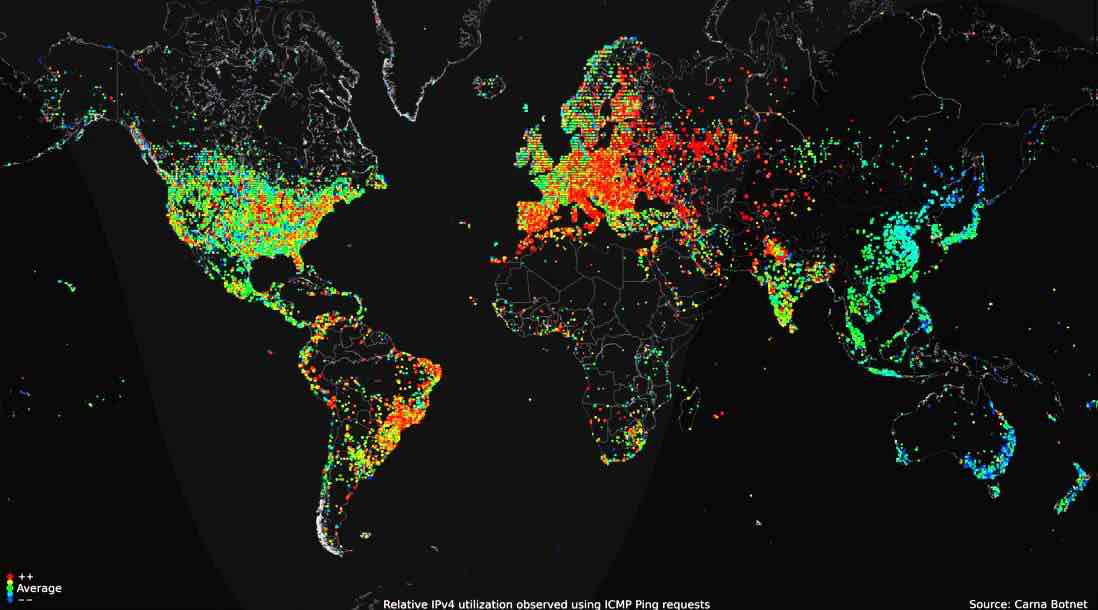
\includegraphics[width=1.2\textwidth]{./images/internet-users-map-1.jpg}}
  ;

\node[expl] 
  (data-NA) 
  at (1,0cm)
  {
\includegraphics[height=0.6cm,keepaspectratio=true]{./images/disc.png}} % 
  ;
\node[expl] 
  (data-CA) 
  at (2.5,1.5cm)
  {
\includegraphics[height=0.6cm,keepaspectratio=true]{./images/disc.png}};
\node[expl] 
  (data-AU) 
  at (10.3,-2.8cm)
  {
\includegraphics[height=0.6cm,keepaspectratio=true]{./images/disc.png}};
\node[expl] 
  (data-EU) 
  at (6.5,2cm)
  {
\includegraphics[height=0.6cm,keepaspectratio=true]{./images/disc.png}};

\node[expl] 
  (user) 
  at (5,0.5cm)
  {
\includegraphics[height=0.6cm,keepaspectratio=true]{./images/user.png}};
  
\draw[arrow]
  (data-NA.south) to[out=270,in=180] ({user}); % [yshift=0.5ex] 
\draw[arrow]
  (data-CA.west) to[out=180,in=180] ({user});  
\draw[arrow]
  (data-AU.north) to[out=90,in=0] ({user});  
\draw[arrow]
  (data-EU.west) to[out=180,in=0] ({user});  
\end{tikzpicture}
% \end{exampleblock}
\end{frame}


\begin{frame}

\frametitle{The Big Data Problem - Process in federated Networks}

\begin{tikzpicture}[
  remember picture,
  overlay,
  expl/.style={draw=orange,fill=orange!30,rounded corners,text width=0.6cm},
 % arrow/.style={red!80!black,ultra thick,->,>=latex}
  line/.style={blue!80!black,ultra thick,-,>=latex}
  arrow/.style={green!80!black,ultra thick,->,>=latex}
]

\node[anchor=south west,inner sep=0]
  (worldmap)
  at (-1,-4.2)
  {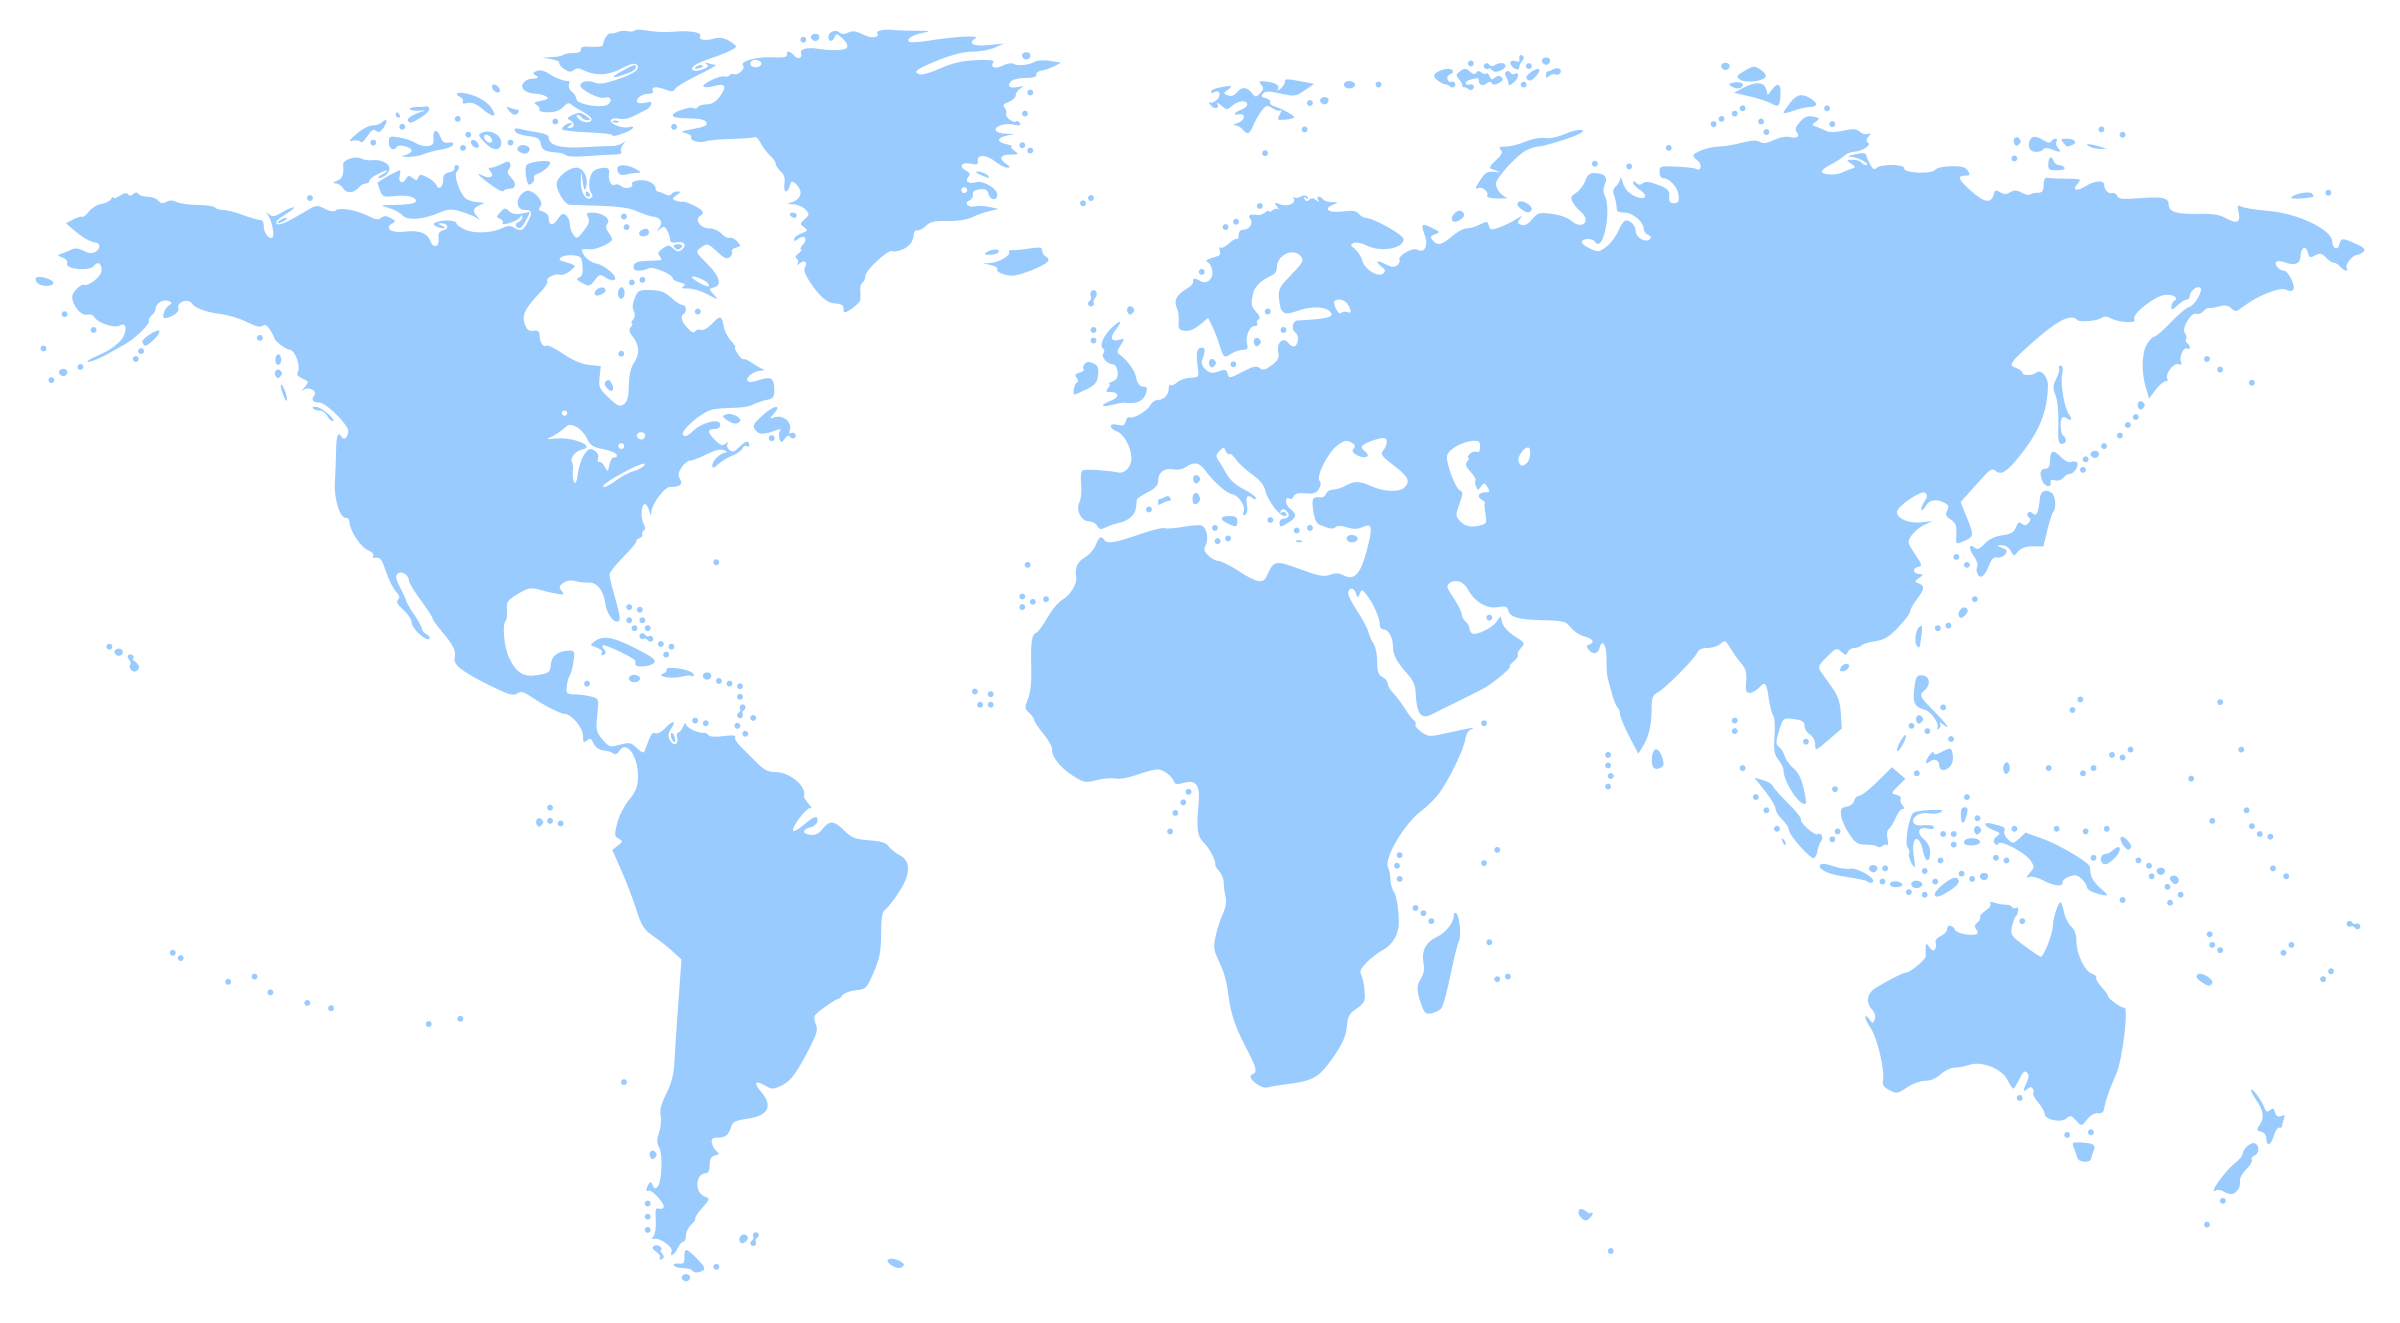
\includegraphics[width=1.2\textwidth]{./images/worldmap}}
  ;
\node[expl] 
  (data-NA) 
  at (1,0cm)
  {
\includegraphics[height=0.6cm,keepaspectratio=true]{./images/disc.png}} % 
  ;
\node[expl] 
  (data-CA) 
  at (2.5,1.5cm)
  {
\includegraphics[height=0.6cm,keepaspectratio=true]{./images/disc.png}};
\node[expl] 
  (data-AU) 
  at (9.5,-3cm)
  {
\includegraphics[height=0.6cm,keepaspectratio=true]{./images/disc.png}};
\node[expl] 
  (data-EU) 
  at (6.5,2cm)
  {
\includegraphics[height=0.6cm,keepaspectratio=true]{./images/disc.png}};

\node[expl] 
  (user) 
  at (5,0.5cm)
  {
\includegraphics[height=0.6cm,keepaspectratio=true]{./images/user.png}};
  
\draw[line]
  (data-NA.north) to[out=90,in=180] ({data-CA});  
\draw[line]
  (data-NA.south) to[out=270,in=180] ({data-AU});  
\draw[line]
  (data-NA.east) to[out=0,in=180] ({data-EU});  
  
\draw[line]
  (data-CA.south) to[out=270,in=180] ({data-AU});  
\draw[line]
  (data-CA.east) to[out=0,in=180] ({data-EU});  

\draw[line]
  (data-AU.north) to[out=90,in=0] ({data-EU});
  
\draw[line]
  (user.east) to[out=0,in=270] ({data-EU});   
\end{tikzpicture}

% \end{exampleblock}

\end{frame}

\begin{frame}

\frametitle{Big opportunity less/least developed countries }

\begin{tikzpicture}[
  remember picture,
  overlay,
  expl/.style={draw=orange,fill=orange!30,rounded corners,text width=0.6cm},
 % arrow/.style={red!80!black,ultra thick,->,>=latex}
  line/.style={blue!80!black,ultra thick,-,>=latex}
  arrow/.style={green!80!black,ultra thick,->,>=latex}
]

\node[anchor=south west,inner sep=0]
  (worldmap)
  at (-1,-4.2)
  {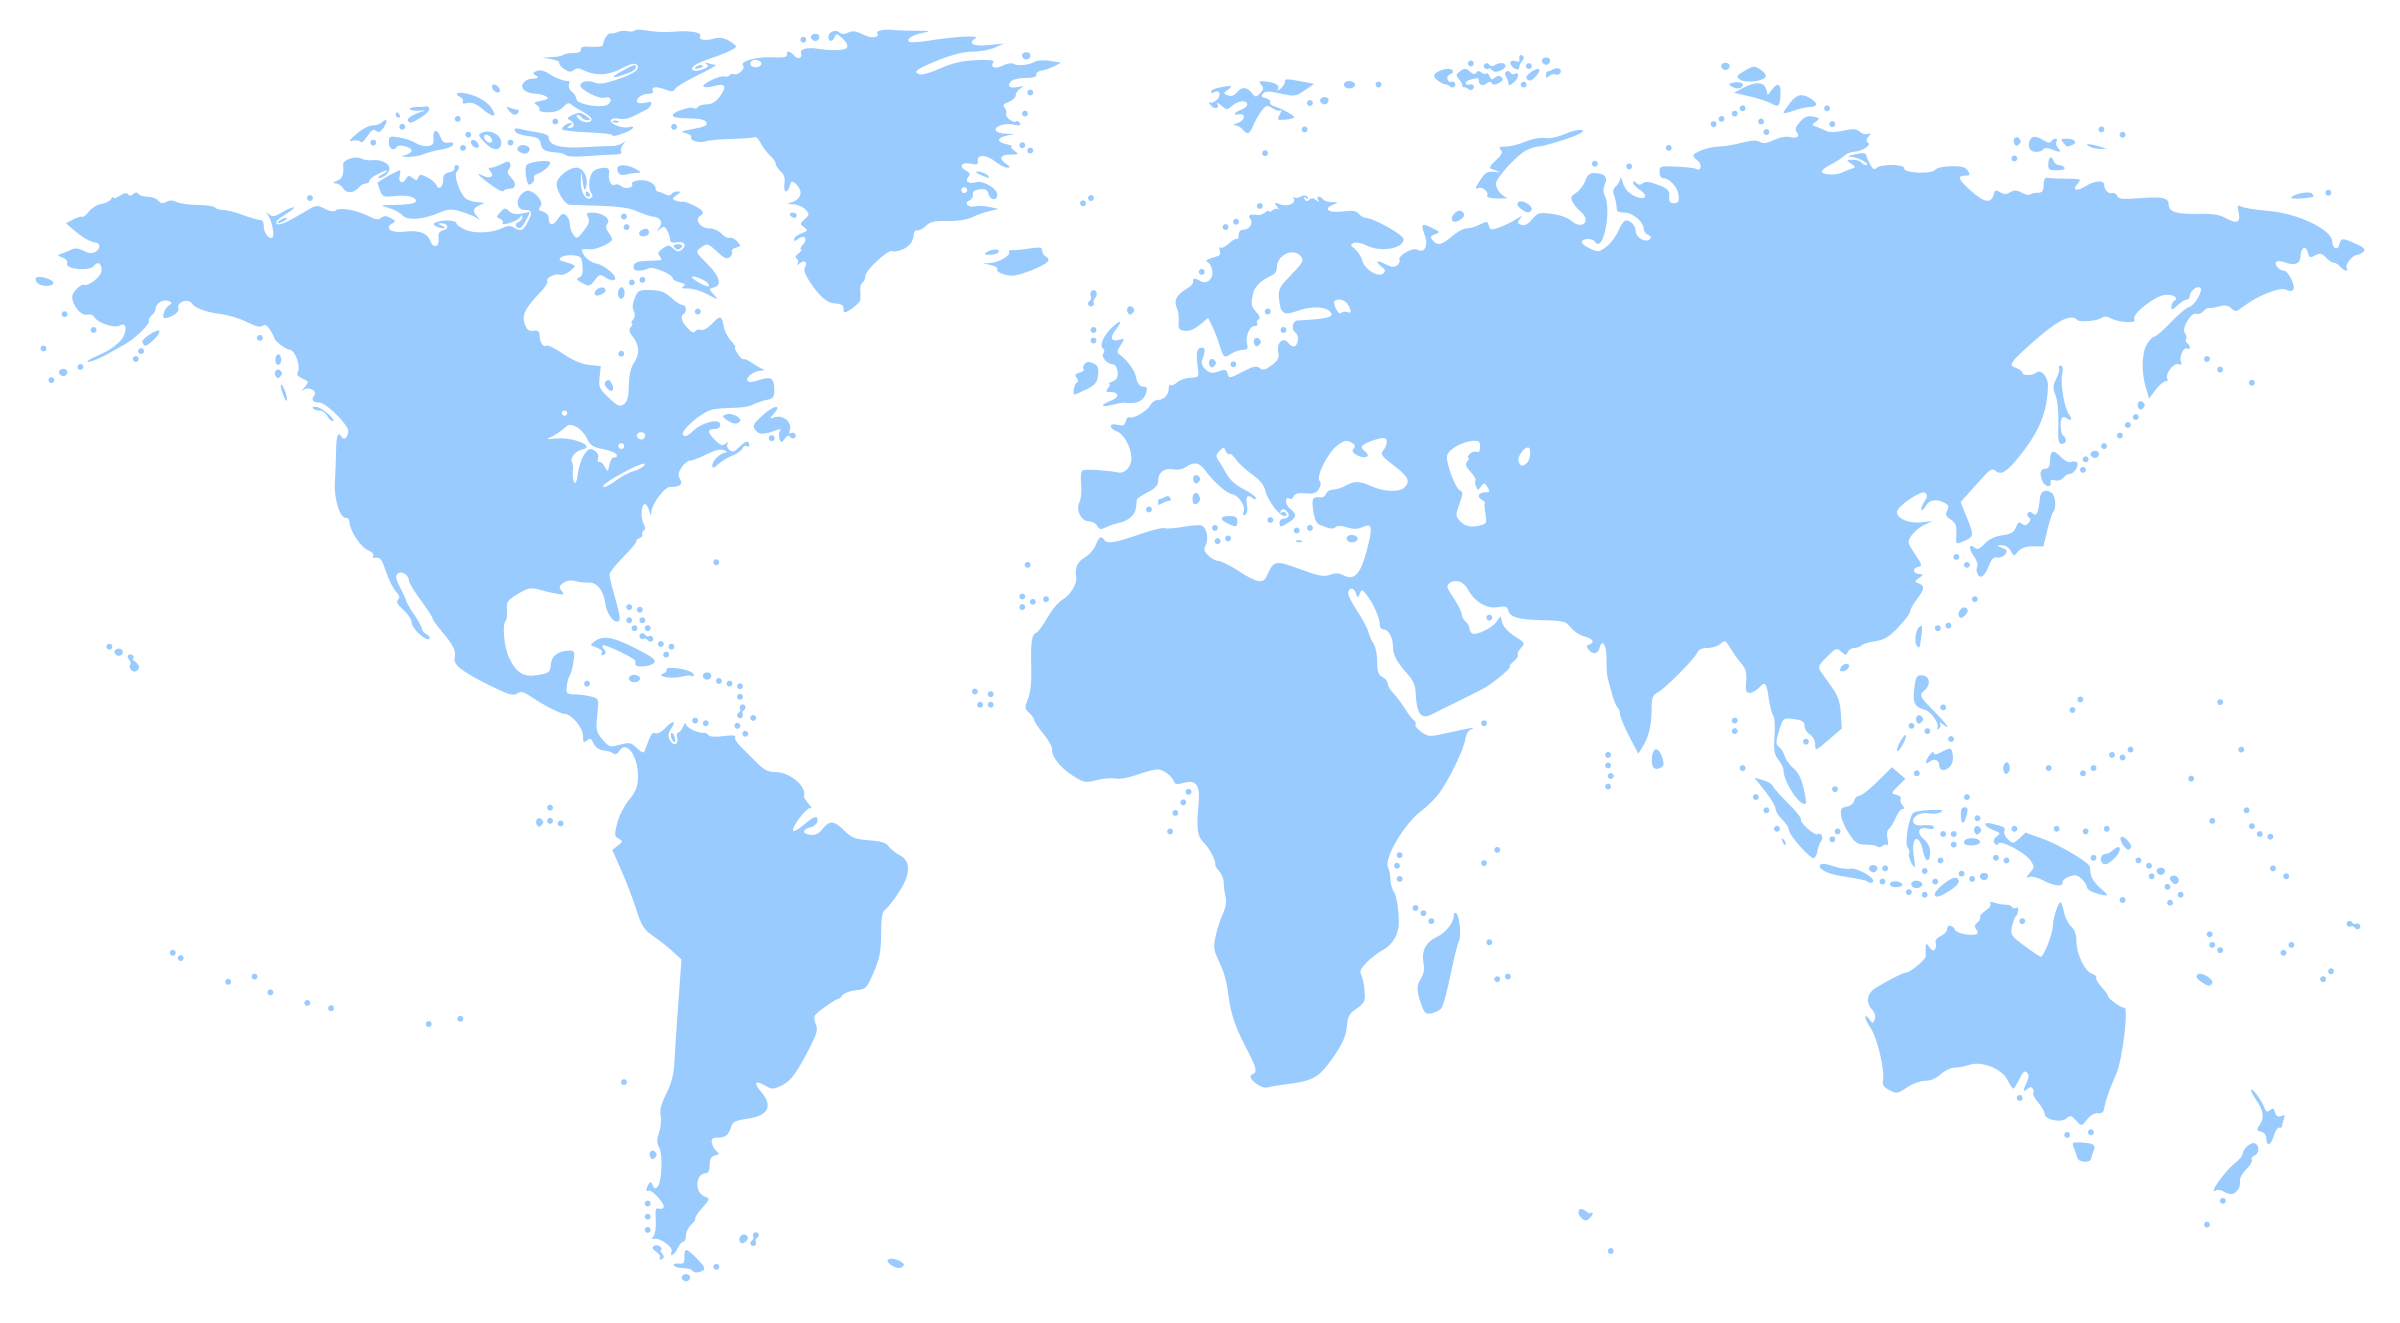
\includegraphics[width=1.2\textwidth]{./images/worldmap}}
  ;
\node[expl] 
  (data-NA) 
  at (1,0cm)
  {
\includegraphics[height=0.6cm,keepaspectratio=true]{./images/disc.png}} % 
  ;
\node[expl] 
  (data-CA) 
  at (2.5,1.5cm)
  {
\includegraphics[height=0.6cm,keepaspectratio=true]{./images/disc.png}};
\node[expl] 
  (data-AU) 
  at (9.5,-3cm)
  {
\includegraphics[height=0.6cm,keepaspectratio=true]{./images/disc.png}};
\node[expl] 
  (data-EU) 
  at (6.5,2cm)
  {
\includegraphics[height=0.6cm,keepaspectratio=true]{./images/disc.png}};

\node[expl] 
  (user) 
  at (5,0.5cm)
  {
\includegraphics[height=0.6cm,keepaspectratio=true]{./images/user.png}};

\node[expl] 
  (user2) 
  at (5.5,-1.5cm)
  {
\includegraphics[height=0.6cm,keepaspectratio=true]{./images/user.png}};
  
\draw[line]
  (data-NA.north) to[out=90,in=180] ({data-CA});  
\draw[line]
  (data-NA.south) to[out=270,in=180] ({data-AU});  
\draw[line]
  (data-NA.east) to[out=0,in=180] ({data-EU});  
  
\draw[line]
  (data-CA.south) to[out=270,in=180] ({data-AU});  
\draw[line]
  (data-CA.east) to[out=0,in=180] ({data-EU});  

\draw[line]
  (data-AU.north) to[out=90,in=0] ({data-EU});
  
\draw[line]
  (user.east) to[out=0,in=270] ({data-EU});   

\draw[line]
  (user2.east) to[out=0,in=270] ({data-EU});   

\end{tikzpicture}


% \end{exampleblock}
\end{frame}



\begin{frame}

\frametitle{Political discourse}  
\definecolor{blue}{HTML}{84CECC}
\definecolor{gr}{HTML}{375D81}


% \begin{tikzpicture}[node distance=0pt,
% 		    SA/.style = {single arrow, draw=blue!40!gray, very thick, fill=blue!20!gray!10,minimum height=1.6*\n1,}]
% \node (n) [text width=0.8\textwidth]
% \path   let \p1 = ($(n.north)-(n.south)$),
%             \n1 = {veclen(\y1,\x1)} in
%         node[SA, rotate=0,  xshift=\n1/2, above=of n.south west] {UNFCCC}
%         node[SA, rotate=0,  xshift=-\n1/2, above=of n.south east] {UNCCD};
% \end{tikzpicture}

%---------------------timeline----------------%

\startchronology[startyear=1990, stopyear=2030, arrow=true]
\chronograduation[periode]{5}

\definechronoevent{UNgen}[textstyle=\bf\raggedright\scriptsize, year=false, align=center, xshift=3cm] 

\definechronoevent{UNFCCC}[textstyle=\bf\scriptsize\raggedright\colorbox{orange!50}, barre=true,  year=false]
\definechronoevent{UNCCD}[textstyle=\bf\scriptsize\raggedright\colorbox{yellow!50}, barre=true, year=false, textwidth=2cm] 
\definechronoevent{UNCBD}[textstyle=\bf\scriptsize\colorbox{green!50}, barre=true, year=false]

% \definechronoevent{UNCBD}[textstyle=\bf, markdepth=110pt, barre=true, colorbox=green, year=true, textwidth=2cm] 
 
\chronoUNFCCC[markdepth=35pt]{1992}{UNFCCC Climate Change}
\chronoUNFCCC[markdepth=21pt]{1995}{Kyoto Protocol} %Emission reduction $5,2 \%$ until 2008-12 
\chronoUNFCCC[markdepth=9pt]{1997}{Copenhagen Agreement} %  Climate Change limit to 2
\chronoUNFCCC[markdepth=21pt]{2011}{Doha Agreement} % second Phase of Kyoto until 2013-20 including reporting system
\chronoUNFCCC[markdepth=9pt]{2015}{Paris Agreement} % Strengthen of Koyoto Protocol\n Climate Change $ <1.5K $ North-South Agreement,transparent technique 

\chronoUNCCD[markdepth=55pt]{1994}{ UNCCD Desertification } %  focus on Africa 
\chronoUNCCD[markdepth=55pt]{2007}{ UNCCD reform } % more Transparency
\chronoUNCCD[markdepth=40pt]{2012}{ LDN until 2030} % Baseline with 3 indices
\chronoUNCCD[markdepth=55pt]{2017}{ Ordos Declaration} % SPI Framework for understanding and monitoring LDN
\chronoUNCBD[markdepth=75pt]{1993}{CBD Biodiversity}
\chronoUNCBD[markdepth=90pt]{2000}{Catachena Protocol} % Control of gen manipulated Organisms
\chronoUNCBD[markdepth=75pt]{2010}{Nagoya Protocol} % Access and Benefit Sharing Aichi Biodiversity Targets 2020

\chronoUNgen[markdepth=130pt, textwidth=2cm]{1992}{United Nations\\ General Assembly\\ RIO} 
\chronoUNgen[markdepth=130pt, textwidth=2cm]{2000}{United Nations\\ World Summit}
\chronoUNgen[markdepth=130pt, textwidth=2cm]{2012}{United Nations\\ RIO20+}

\chronoUNgen[markdepth=150pt]{1990}{IPCC AR1}
\chronoUNgen[markdepth=150pt]{1995}{IPCC AR2}
\chronoUNgen[markdepth=150pt]{2001}{IPCC AR3}
\chronoUNgen[markdepth=150pt]{2007}{IPCC AR4}
\chronoUNgen[markdepth=150pt]{2014}{IPCC AR5}
\chronoUNgen[markdepth=150pt]{2020}{($\sim$IPCC R6)}

\chronoUNgen[markdepth=140pt]{2017}{\textbf{Global Land Outlook}}

\chronoperiode[textstyle=\raggedleft\colorbox{gr!50}, color=gr, startdate=false, bottomdepth=0pt, topheight=9pt, textdepth=-15pt,dateselevation=8pt, stopdate=false]
{2000}{2015}{Millenium Goals}

\chronoperiode[textstyle=\colorbox{blue!50}, color=blue, startdate=false, 
bottomdepth=0pt, topheight=9pt, textdepth=-15pt, dateselevation=0pt, stopdate=false]
{2015}{2030}{ SDGs }

\stopchronology
\end{frame}


\begin{frame}

\frametitle{Cherry Picking aspects of the Paris Agreement (COP21)}

\textbf{Article 6 Paragraph 2:}\\
'Parties shall, where engaging on a voluntary basis in cooperative approaches ...‘\\

\textbf{Article 6 Paragraph 8.:}\\
'Parties recognize the importance of integrated, holistic and balanced non-market approaches being available to Parties to assist in the implementation of their nationally determined contributions,...'\\

\textbf{Article 7 Paragraph 7:}\\
Parties acknowledge that adaptation action should follow a country-driven, gender-responsive, participatory and fully transparent approach, ...'\\

\textbf{Article 10 Paragraph 1:}\\
 'Parties share a long-term vision on the importance of fully realizing technology development and transfer in order to improve resilience to climate change and to reduce greenhouse gas emissions.\\

\textbf{Article 10 paragraph 2:}\\
 'Parties, noting the importance of technology for the implementation of mitigation and adaptation actions under this Agreement and recognizing existing technology deployment and dissemination efforts, shall strengthen cooperative action on technology development and transfer.‘\\
\end{frame}

\begin{frame}{Shift of principles for knowledge management }
    \begin{figure}[ht]
%         \begin{minipage}[b]{0.55\linewidth}
            \centering
            \includegraphics[height=0.7\textheight]{./images/Copyright_copyleft.jpg}            
            \caption{copyleft}
            \label{fig:copyleft}
%         \end{minipage}
%         \hspace{0.5cm}
%         \begin{minipage}[b]{0.35\linewidth}
%             \centering
%             \includegraphics[width=\textwidth]{./images/copyright.png}
%             \caption{Copyright}
%             \label{fig:copyright}
%         \end{minipage}
    \end{figure}
\end{frame}


\begin{frame}

\frametitle{Organizations Landscape}

\begin{figure}[ht]
\centering

\smartdiagramset{border color=none,
uniform color list=blue for 3 items, % teal!70!black
module shape= circle, 
module minimum height=2.5cm,
module minimum width=2.5cm,
circular distance=2.5cm,
font=\Huge\sffamily\bfseries, 
text width=5em,
text color=black,
arrow line width=5pt,
arrow style=<->,
additions={
additional item font=\sffamily\bfseries\color{black!70},
additional item offset=1.5em,
additional item height=0em,
additional item text width=7em,
% additional arrow color=teal!40,
% additional arrow line width=4pt,
}}
\smartdiagramadd[circular diagram:clockwise]{DATA, DAC, FOSS}{
right of module1/ Group of Earth observation, 
right of module2/Development Agencies Community,
left of module3/Open Spatial Consortium}
% 
% 
% \smartdiagramconnect{-}{module1/additional-module2}
% \smartdiagramconnect{<-}{module3/additional-module3}
% \smartdiagramconnect{<->}{module3/additional-module4}
% \smartdiagramconnect{->}{module2/additional-module5}
% 
\end{figure}
\end{frame}

\begin{frame}{High Performance Computation for Sustainable Development}
\begin{figure}[ht]
    \begin{minipage}[b]{0.55\linewidth}
	\centering
	\includegraphics[width=\textwidth]{./images/datacenter.png}            
	\caption{High Performance Computer}
	\label{fig:a}
    \end{minipage}
    \hspace{0.5cm}
    \begin{minipage}[b]{0.35\linewidth}
	\centering
	\includegraphics[width=\textwidth]{./images/SDGs.png}
	\caption{Sustainable Development Goals}
	\label{fig:b}
    \end{minipage}
\end{figure}


Further reading:\\ 
\href{https://medium.com/birdhouse-newsletter/cyber-structures-for-sustainable-development-74b3e4deeff1}{Cyber-structures for sustainable development} 

\href{https://medium.com/birdhouse-newsletter/the-it-landscape-for-climate-services-4e21c32c4ffb}{The IT Landscape for Climate Services} 

\end{frame}
